\chapter{Silicon detectors basics} %PREELIMINARY TITLE % (fold)
%I should probably talk about leakage current as well
\label{chap:detector}

In general, a solid state detector consists of an enclosed volume, filled with a material in
which free charge carriers can be generated by an incident particle. This volume
is connected to a power supply that provides a  potential difference between two
points inside the volume. The potential difference induces the drift of the
carriers. The current induced by this movement is then picked on electrodes,
amplified and processed by some front end electronics.

Even though this general concept of particle detector holds true for almost
every detector in use nowadays the implementation of this concept varies greatly
depending on the material from which the detector is constructed. In the
following sections we will summarise the operational principles of silicon
detectors

\section{P-N Junction}

Silicon is a semiconductor material. Its electrical properties can be modified
by adding controlled impurities to the lattice; this process is called doping.
There are two main types of dopants used: acceptor impurities and donor
impurities (see Figure \ref{fig:dopingSi}). Phosphorous is a typical donor dopant. It has 5 electrons in its
outer shell. When added to the Si lattice, the extra electron is lightly bound.
In the energy-momentum representation, the P atom introduces an energy close to
the conduction band. Phosphorous doped silicon is known as n-type silicon. 

\begin{figure}[H]
	\centering
	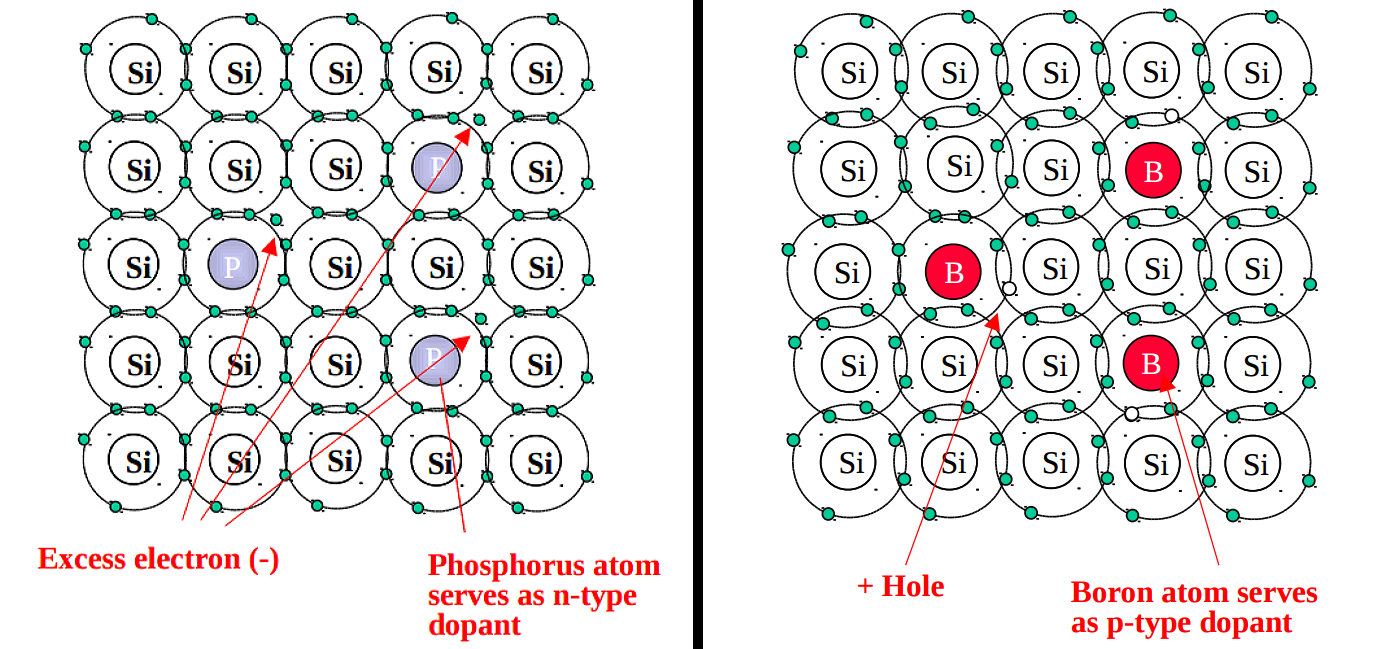
\includegraphics[width=0.8\textwidth]{Dopants_Si.png}
	\caption{Sketch of doped silicon for both $n$ (left) and $p$ (right) dopant types. For $n$-type dopant Phosphorous is shown as example; Boron is used as example of $p$-type dopant.}
	\label{fig:dopingSi}
\end{figure}

On the other hand, Boron is an example of acceptor dopant. Boron has 3 electrons
in its outer shell. When Boron is made to substitute a Silicon atom in the
lattice, an electron from a nearby Silicon atom will fill this deficiency. The
Si atom contributing with the electron, will have a hole in its outer shell,
that can be occupied with another electron from a neighbour atom. From a general
perspective, the "hole" associated to the original Boron has now moved to
another Silicon atom. This motion of a "hole" illustrates the conduction due to
holes in a p-type doped Silicon.

These donor (or acceptor) levels introduced by impurities are very close to the
conduction (valence) band. Energies of the order of $k_B T$ (with $k_B$ being 
Boltzman's constant and $T$, temperature) at room temperature are enough to 
excite electrons from the dopant level into the conduction band (from the 
valence band into the impurity level). These addition of dopants to 
Silicon improves electrical conductivity of Silicon by orders of magnitude.  

In a real semiconductor, there are impurities of both types, despite the fact
that one kind of them can be majority. The difference between the number of
donor impurities ($N_D$) and acceptor impurities ($N_A$) dictates whether the
material is $p$-doped ($N_A > N_D $) or n-doped ($N_D > N_A$). This difference
is called $N_{eff}$, or the effective doping concentration and is usually 
expressed in cm$-3$

When $n$-type Silicon is put in contact with $p$"-type a pn-junction is formed.
Due to the concentration difference, electrons from the n-type will diffuse to
the p-type material, while holes from the $p$-side will diffuse into the
n-material. While doing so, an electric field appears from the n-type to the
p-type material due to the fixed spatial charges (ionized atoms). This electric
field will then stop diffusion of free carriers. The ionised atoms in the
silicon lattice cannot effectively move from their initial positions. The region
depleted of lightly bound (free) charge carriers is called the depletion zone.
Note that this region exists even in the absence of an external potential. The
charge separation between the 2 oppositely doped volumes leads to an electrostatic
potential. This voltage difference is called built-in
voltage. If now a potential difference is applied such that the n-side is made
positive with respect to the p-side, the depleted region will increase. This is
called reverse biasing, and it is the electrostatic configuration needed to 
operate a detector.

\subsection{Effective space charge distribution (Neff)} 
%Talk equations and introduce the concept of Neff and its shape in a non-irradiated silicon detector

The electrical properties of the $p-n$ junction can be derived from Poisson equation. 
\begin{equation}
\nabla^2 \phi = \frac{\rho(x)}{\epsilon} 
\label{eq:poisson}
\end{equation}

Where $\phi$ is the electrostatic potential, $\epsilon$ the absolute
permittivity of silicon and $\rho(x)$ is the space charge distribution as a
function of position (assuming here a 1D problem).

The value of $N_{eff}$ determines the potential and electric field in a
non-irradiated detector. This value is constant (and equal to the doping of the
bulk). For now, we will focus on the non-irradiated case. We consider a junction
located at $x=0$, being $-x_p$ and $x_n$ the extremes of the depleted zone.

It is important to note that since both the $n$-doped and $p$-doped silicon were
electrically neutral at the beginning and no charge has been created or
destroyed in the process of creating the junction, the material as a whole will
remain neutral which means the total amount of charge has to be equal on both
sides. This leads to a the mass action law, described as \[N_A x_p = N_D x_n\] 
For silicon particle detectors, one of the two sides is doped higher with
respect to the other (e.g.: $N_A >> N_D$  so that the depletion zone is almost
entirely on one side of the junction ($x_n >> x_p$). 

With this configuration the width of the depleted zone ($w$) is $w \approx x_p$.
When Poisson's equation is solved for $\rho = const$ the resulting electric
$\nabla \phi = -\overrightarrow {E}$ field is linear with the distance to the $p-n$
junction. In a typical detector configuration (where $w \approx x_{p/n}$) this
means there is an electric field across the whole active volume of the detector
(depleted area) in which any carrier created will move by drift. 


\section{Detector configuration}
\label{sec:detConfig}

If the detector is partially depleted, then part of the detector will not be
efficient to detect ionisation after a crossing particle. Indeed, the free
charge carriers produced will recombine in the undepleted bulk. Therefore, the
full detector needs to be depleted for optimal operation. For this purpose a
bias voltage ($\vias$) is applied following the same polarity as the built-in
potential $V_0$ and increases the depleting effect of the $p-n$ junction
therefore increasing the active volume of silicon. 

Solving Poisson equation with \vias as contour condition, the following
expression is obtained: 

\begin{equation}
w = \sqrt{\frac{2\epsilon V_{bias}}{\epsilon_0 N_D}}
\label{eq:widthVias}
\end{equation}

What this equation shows is that the depleted volume increases as the square
root of the bias voltage and that it is inversely proportional to the doping of the
bulk. Effectively, the higher the doping, the more difficult it is to deplete the
device with a fixed voltage. 

The silicon pad detector remains one of the most important detector designs,
particularly in research, due to its simplicity. It is composed of a thin
(typically ~1$\mu$m) layer of very highly doped silicon, called the implant,
that sits on top of a thicker (typically 300$\mu$m) piece of silicon with a
lower volume density of dopants, called the bulk. Silicon particle detectors are
bulk devices. Connection to the electrical circuit that provides the \vias and
performs read-out of the signal is done by means of metal electrodes on the top
part of the pad and an ohmic contact with a metal in the back. 

\section{Signal Generation: Ramo's Theorem} % No es Sergio Ramos, es otro Ramo's
\label{sec:Ramo}
%-> Gran Frase

The depleted part of the silicon detector is the volume in which free
charge carriers are created by ionisation and then drift inducing an electrical
current in the electrodes. This instantaneous current can be time resolved and
recorded for later analysis. This is the basis of the Transient Current
Technique that will be explained further on in this report. The induced current
in a system of electrodes can be readily calculated using Ramo-Shockely theorem.


The Ramo-Shockely Theorem states that the current induced by a moving charge in
a system of electrodes is proportional to its charge, velocity and to a
magnitude called weighting field, that quantifies how the charge couples to an
electrode. This weighting field is a purely geometrical factor. For instance,
for a pad detector, the weighting field is a constant. In a microstrip detector
the weighting field is very small when the charge is far from the electrode and
is more important as it comes closer. Mathematically, the expression for the
induced current is

\begin{equation}
	i = q \cdot \overrightarrow {v} \cdot \overrightarrow {E_{W}}
	\label{eq:ramo} 
\end{equation} 

where $q$ is the charge, $\overrightarrow {v}$ the drift velocity and $\overrightarrow E_{W}$ the weighting
field. In 1D the vectors are replaced by their magnitudes.

For a system where more than one particle is moving and thus inducing current in
the circuit, the total current can be written as the sum of each individual
contribution. If all the charge carriers have the same charge, as it is in the
case for electrons and holes, drifting inside the silicon volume, then equation
(\ref{eq:ramo}) can be re-written as:

\begin{equation}
	I = q \cdot \sum_{n=1}^{N} \overrightarrow {v_n}\overrightarrow {E_{W}} 	\label{eq:ramoTot} 
\end{equation} 

Note that though the charge for electrons and holes is opposite, they move as
well in opposite directions and the currents from both add. The drift velocity 
is proportional to the electric field, the proportionality factor being 
the mobility. The mobility is only constant for low electric fields. Then 
it reduces as $1/E$. Like this, the drift velocity increases linearly with 
the field until a certain limit, where it reaches a plateau. The drift 
velocity thus saturates when the speed of the carriers equals the thermal 
speed of the electrons. Typically electron mobilities ($ \mu_e $) are taken to 
be referred to the conduction band unless otherwise specified. Conversely, 
hole mobilities ($ \mu_h $) are taken to be referred to the valence band 
by default. Putting all this together we arrive at 

\begin{equation}
	I = q \cdot \sum_{n=1}^{N} \mu_n(E) \overrightarrow {E} \cdot \overrightarrow {E_{W}} 
\label{eq:ramoMob}
\end{equation}

